\section{Hardware design}

In this section, the hardware design and implementation of the micromouse robot are described. First, the corresponding electrical circuit, known as scematic, is broken down to its components and thoroughly presented. In the next subsection, the actual components chosen for the hardware implementation are listed. The model for the final Printed Circuit Board (PCB) follows right after, where the chosen electrical components are placed in the computer model. Last, but not least, the protective casing for the micromouse is described.

\subsection{Schematic and Components Description}

The first step in the development of the hardware is the drawing of the electrical circuit. The realization of a moving micromouse demands for the combination of a variety of components connected to each other. Exactly this is described in the so called schematic of the circuit, which resembles a drawing on paper. 
The schematic of the micromouse can be seen in Fig. \ref{fig:schematic_overview}.

\begin{figure}[htb]
    \centering
    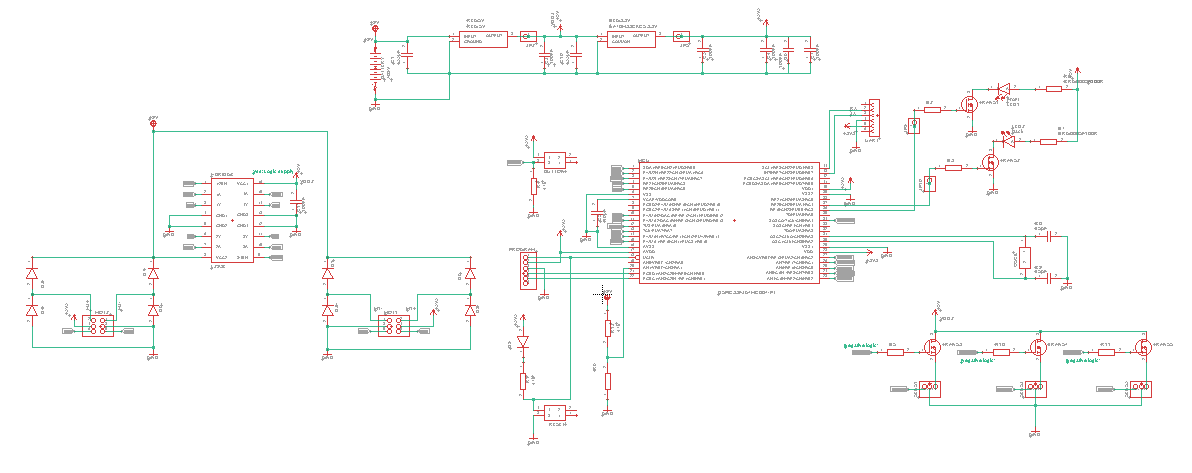
\includegraphics[width=1\textwidth]{figures/hardware/Schematic.PNG}
    \caption{Schematic overview of the micromouse}
    \label{fig:schematic_overview}
\end{figure}

This can look intimidating at first and definitely not readable in such a miniature picture. So, let's break it down to its components and describe its sub-circuits.
With the exception of the first subsection, the components will be presented from left to right and from top to bottom, so that the reader may always refer to the overview schematic to get a clear picture of a component's relation to the whole.

\FloatBarrier

\subsubsection{Microcontroller (MCU)}

Describe pins locations and assignment. Include a table, like the one in our excel spreadsheet.
Describe the labels utility in Eagle. 
Describe the pins electrical limitations according to the datasheet.

\begin{figure}[htb]
    \centering
    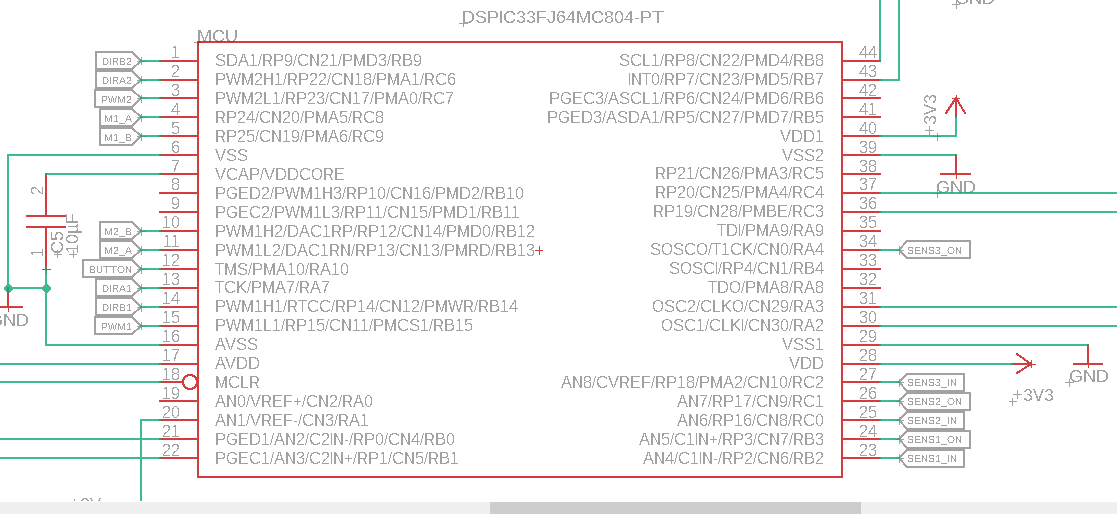
\includegraphics[width=0.8\textwidth]{figures/hardware/MCU.PNG}
    \caption{The dsPIC33FJ64MC804 microcontroller}
    \label{fig:mcu}
\end{figure}

\FloatBarrier

\subsubsection{Votage Regulators}

Describe the different votages needed in the circuit.
Describe the role of a voltage regulator.
Describe the need for decoupling capacitors.

\begin{figure}[htb]
    \centering
    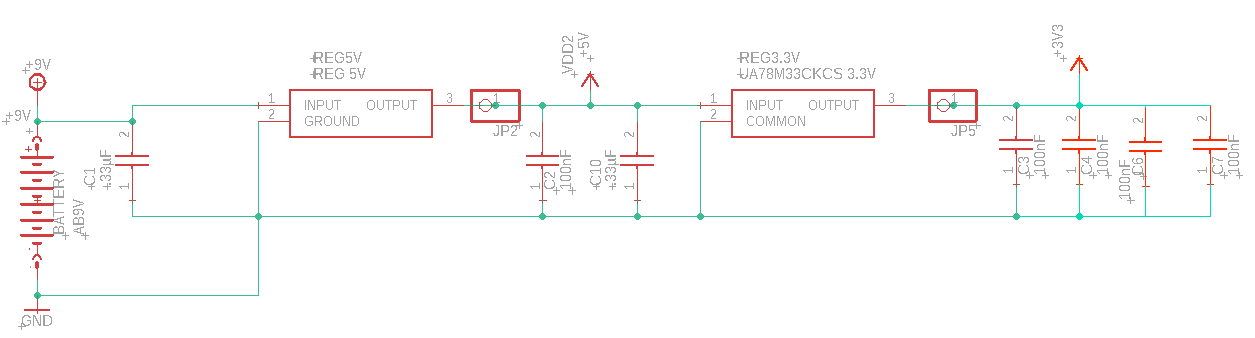
\includegraphics[width=0.8\textwidth]{figures/hardware/VoltageandCapacitors.PNG}
    \caption{The battery and voltage regulators}
    \label{fig:battery}
\end{figure}

\FloatBarrier


\subsubsection{H-Bridge and Motors}

Describe the motors pins, with picture.
Describe the need for an H-bridge and its functionality, with picture.
Describe the escape diodes and their functionality.

\begin{figure}[htb]
    \centering
    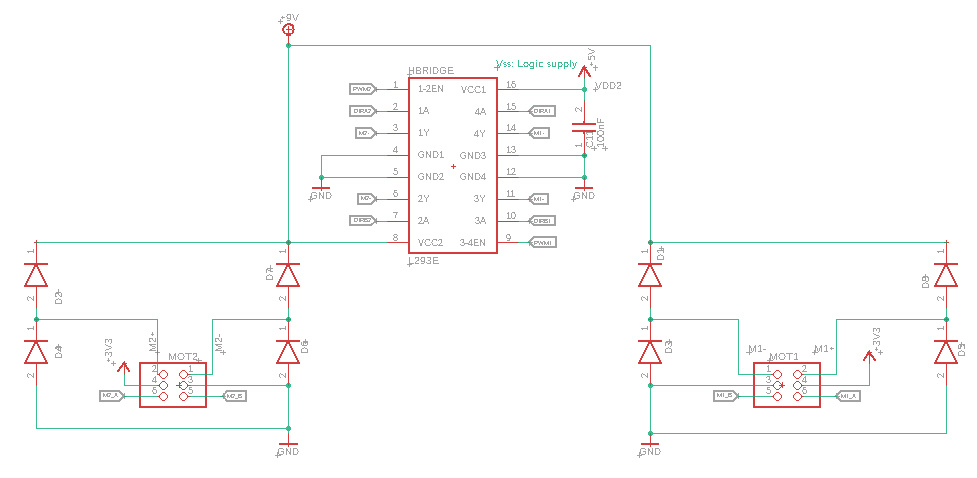
\includegraphics[width=0.8\textwidth]{figures/hardware/MotorsandHBridge.PNG}
    \caption{The motors and the H-bridge}
    \label{fig:motors}
\end{figure}

\FloatBarrier


\subsubsection{Extra Button}

Describe the need for an extra button and the pull-down resistor and value choice.

\begin{figure}[htb]
    \centering
    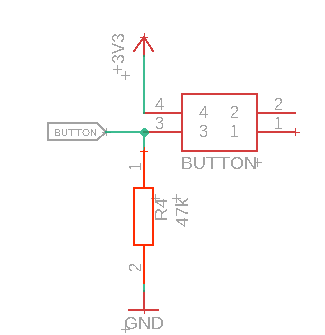
\includegraphics[width=0.8\textwidth]{figures/hardware/Button.PNG}
    \caption{An extra button for input}
    \label{fig:button}
\end{figure}

\FloatBarrier


\subsubsection{Programmer}

Describe the usage of the programmer.

\begin{figure}[htb]
    \centering
    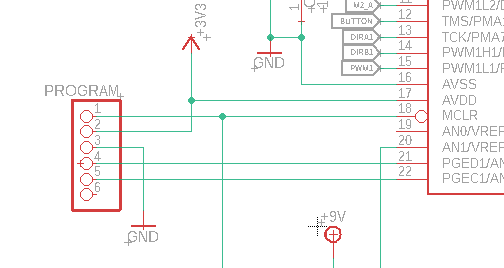
\includegraphics[width=0.8\textwidth]{figures/hardware/Programmer.PNG}
    \caption{The programmer}
    \label{fig:programmer}
\end{figure}

\FloatBarrier


\subsubsection{Reset Button}

Describe the need for a reset button.
Describe the negative logic and pull-up resistor.

\begin{figure}[htb]
    \centering
    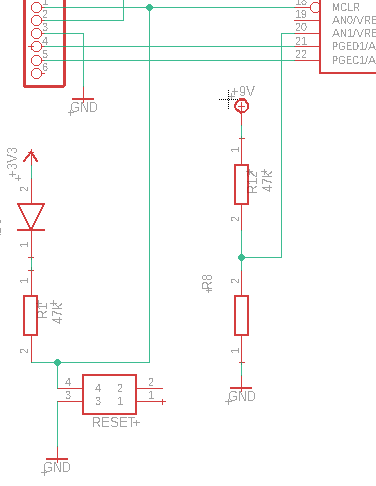
\includegraphics[width=0.8\textwidth]{figures/hardware/MCLRandBatteryMeasurement.PNG}
    \caption{The reset button and the battery voltage measurement circuit}
    \label{fig:reset}
\end{figure}

\FloatBarrier


\subsubsection{Battery Measurement}

Describe the need for measuring the battery voltage level
and adjusting the PWM accordingly. 
Describe the concept of voltage divider and the values chosen.


\subsubsection{Universal Asynchronous Communication (UART)}


Describe the need for UART, to issue commands at will.

\begin{figure}[htb]
    \centering
    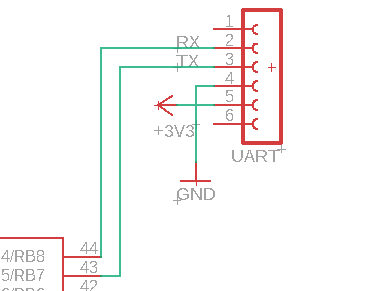
\includegraphics[width=0.8\textwidth]{figures/hardware/UART.PNG}
    \caption{The UART module}
    \label{fig:uart}
\end{figure}

\FloatBarrier


\subsubsection{LEDs}

Describe the need for mechanical stability and the usage of LEDs. Say why we want to blink them.
Describe why transistors are needed and briefly the way they are connected.

\begin{figure}[htb]
    \centering
    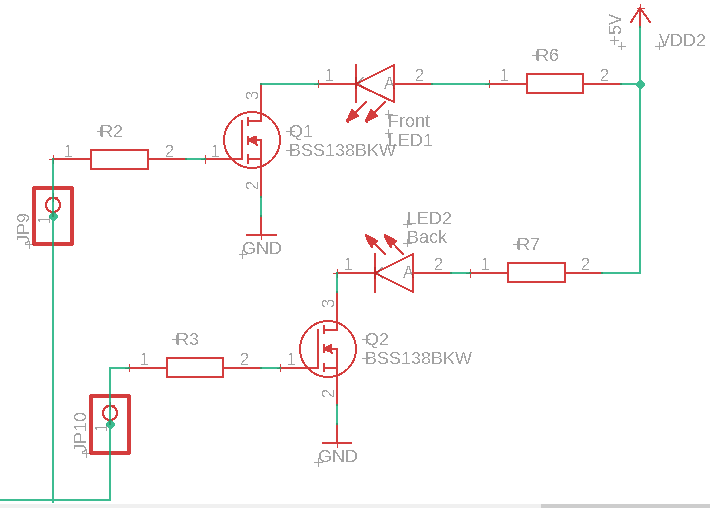
\includegraphics[width=0.8\textwidth]{figures/hardware/LEDs.PNG}
    \caption{The LEDs used for mechanical stability}
    \label{fig:leds}
\end{figure}

\FloatBarrier


\subsubsection{Oscillator}

Describe the choice for an external oscillator and the need for capacitors (mcu datasheet).

\begin{figure}[htb]
    \centering
    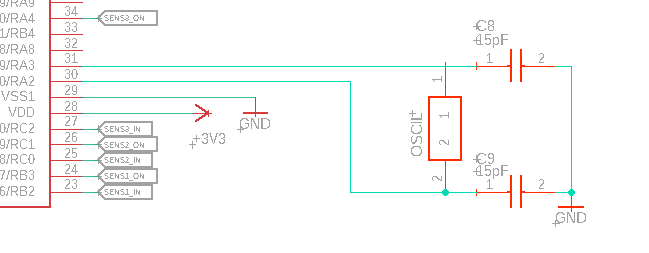
\includegraphics[width=0.8\textwidth]{figures/hardware/Oscillator.PNG}
    \caption{The external oscillator}
    \label{fig:oscillator}
\end{figure}

\FloatBarrier


\subsubsection{Distance Sensors}

Describe the need for sensors and the way they are connected.
Explain why we chose to have transistors there.

\begin{figure}[htb]
    \centering
    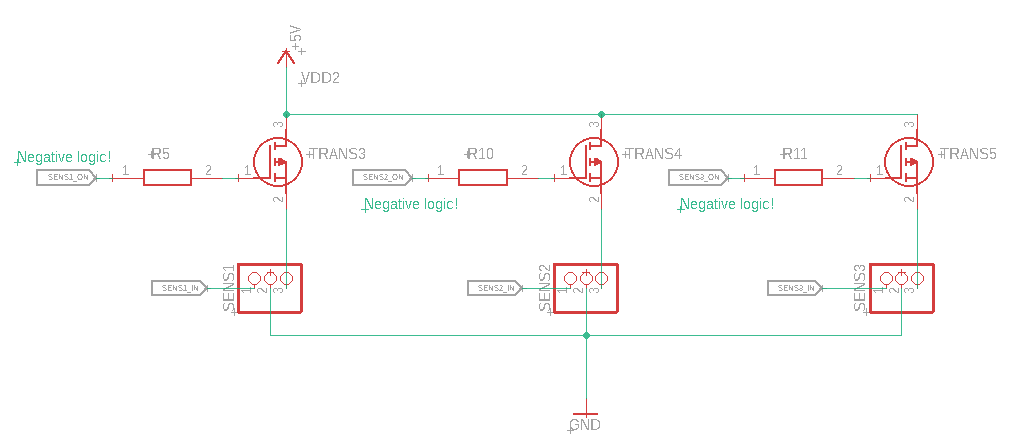
\includegraphics[width=0.8\textwidth]{figures/hardware/DistanceSensors.PNG}
    \caption{The distance sensors}
    \label{fig:sensors}
\end{figure}

\FloatBarrier



\subsection{Components}

List the actual components we ordered.
No need to explain the values for resistors and capacitors.
Explain specific choices if needed.


\subsection{Printed Circuit Board (PCB)}

Comment on the restrictions of the PCB, dimensions and shape.
Explain the components' placement choice.
Describe the concept of 2 layers and via points.
Describe the concept of ground plane.
Comment on electrical noise, its sources and why it doesn't really matter in our case.

\begin{figure}[htb]
    \centering
    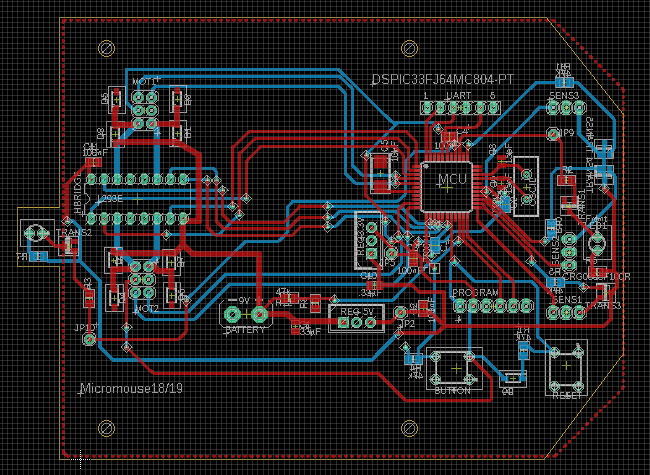
\includegraphics[width=0.8\textwidth]{figures/hardware/PCB.PNG}
    \caption{The PCB with both top and bottom tracks visible}
    \label{fig:pcb}
\end{figure}

\begin{figure}[htb]
    \centering
    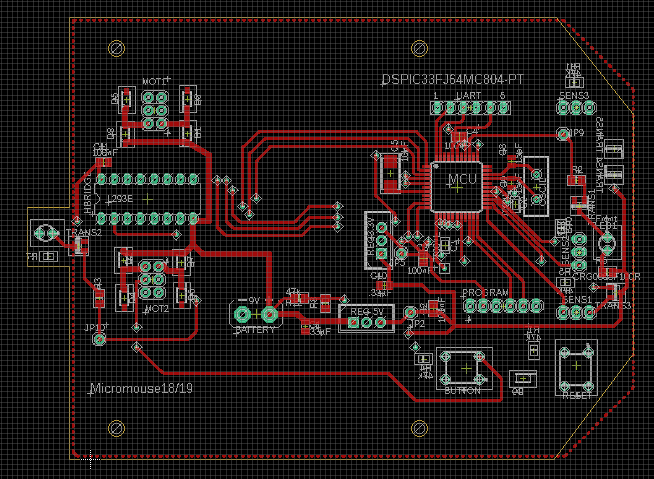
\includegraphics[width=0.8\textwidth]{figures/hardware/PCB_Top.PNG}
    \caption{The PCB with only top layer tracks visible}
    \label{fig:top}
\end{figure}

\begin{figure}[htb]
    \centering
    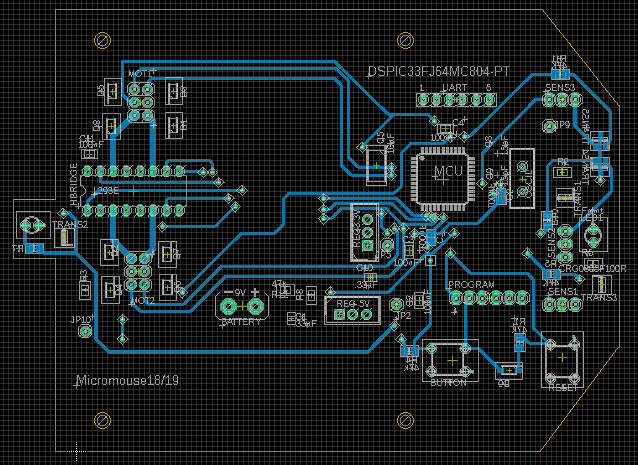
\includegraphics[width=0.8\textwidth]{figures/hardware/PCB_Bottom.PNG}
    \caption{The PCB with only bottom layer tracks visible}
    \label{fig:bottom}
\end{figure}

\begin{figure}[htb]
    \centering
    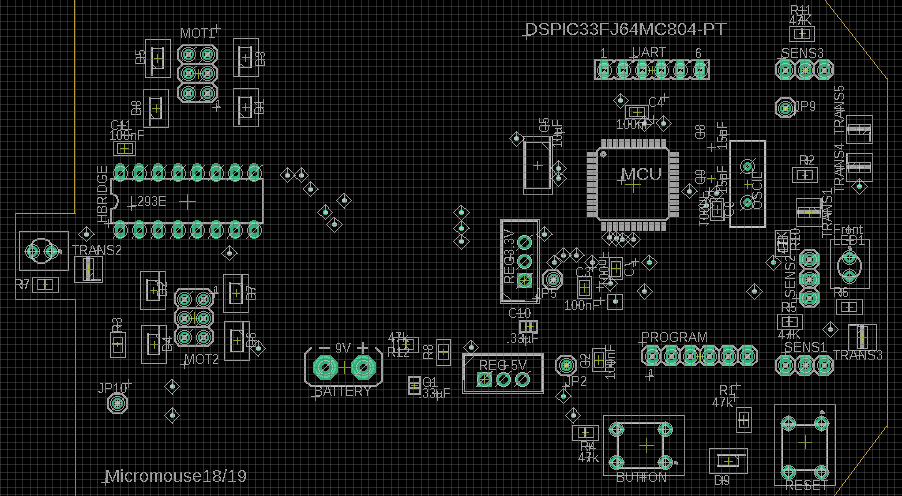
\includegraphics[width=0.8\textwidth]{figures/hardware/PCB_Components.PNG}
    \caption{The PCB without tracks, only components visible}
    \label{fig:comp}
\end{figure}

\begin{figure}[htb]
    \centering
    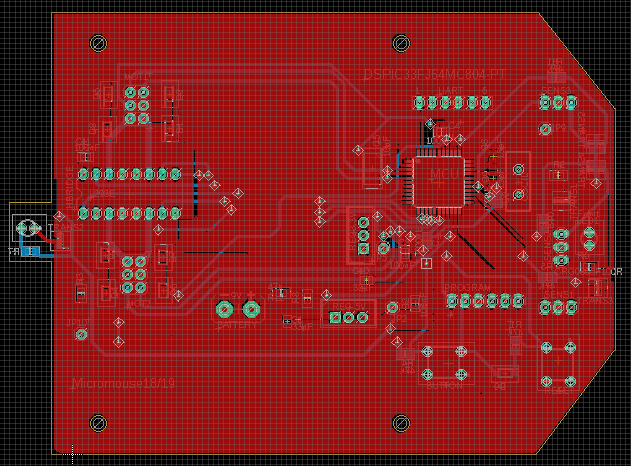
\includegraphics[width=0.8\textwidth]{figures/hardware/PCB_Grounded.PNG}
    \caption{The PCB with the ground plane visible}
    \label{fig:gnd}
\end{figure}

\FloatBarrier

\subsection{Casing}

Present the need for casing.
Describe it.
Present necessary pictures.
Describe important calculations.






